% Fig. 2 -- L4.7 operating characteristic.
% Included by paper/icc_main.tex via \input.
%
% This REPLACES the 17-class coverage matrix, which gave the largest visual allocation to
% the weakest result -- a matrix of assertions firing on inputs shaped to trip them.
%
% AXIS NOTE. An earlier version plotted the data at x = 5*ICC (the effect SD) while ticking the
% axis in ICC at x = 0,1,2,3 -- so the ticks labelled 0.5 and 0.8 sat at ICC 0.4 and 0.6, the
% curve ran past the end of its own axis, and reading power off the tick labelled 0.8 gave 0.87
% against a caption claiming 1.00. The x coordinate is now ICC itself. Keep it that way: if a
% point is added, give it an ICC coordinate, never an effect size.
%
% Every number below is read from evaluation/results/l47_power_curve.json and the
% l47_calibration block of final_summary.json, both regenerated by `make matrix`.
\begin{figure}[!t]
\centering
\resizebox{\columnwidth}{!}{%
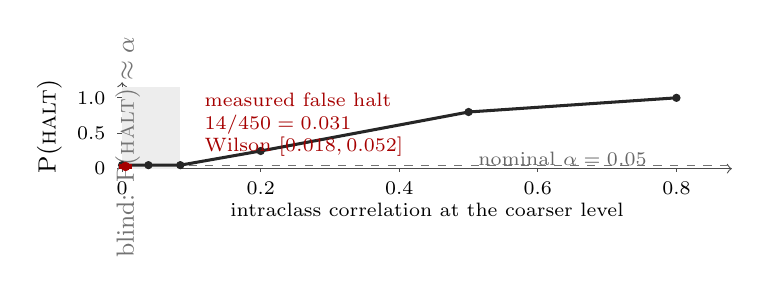
\begin{tikzpicture}[font=\footnotesize,x=88mm,y=9mm]
% axes. x runs past the last datum (ICC 0.8) so the curve ends inside its own axis.
\draw[->,black!70] (0,0) -- (0.88,0);
\draw[->,black!70] (0,0) -- (0,1.22);
\foreach \x/\lab in {0/{0}, 0.2/{0.2}, 0.4/{0.4}, 0.6/{0.6}, 0.8/{0.8}}
  {\draw[black!70] (\x,0) -- (\x,-0.04); \node[below,font=\scriptsize] at (\x,-0.05) {\lab};}
\foreach \y/\lab in {0/{0}, 0.5/{0.5}, 1/{1.0}}
  {\draw[black!70] (0,\y) -- (-0.008,\y); \node[left,font=\scriptsize] at (-0.010,\y) {\lab};}
\node[below,font=\scriptsize,align=center] at (0.44,-0.34)
  {intraclass correlation at the coarser level};
\node[rotate=90,font=\small] at (-0.105,0.6) {P(\textsc{halt})};
% low-correlation region: power is indistinguishable from size
\fill[black!7] (0,0) rectangle (0.084,1.15);
\node[font=\small,text=black!55,rotate=90,anchor=south] at (0.040,0.30)
  {blind: P(\textsc{halt}) $\approx\alpha$};
% nominal alpha reference
\draw[dashed,black!55] (0,0.05) -- (0.88,0.05);
\node[font=\scriptsize,text=black!60,anchor=west] at (0.50,0.135)
  {nominal $\alpha=0.05$};
% measured curve. x is ICC, y is measured P(HALT) over 40 seeds per point.
\draw[line width=1.1pt,black!85]
  (0.000,0.05) -- (0.010,0.05) -- (0.038,0.05) -- (0.084,0.05)
  -- (0.200,0.25) -- (0.500,0.80) -- (0.800,1.00);
\foreach \x/\y in {0.000/0.05, 0.038/0.05, 0.084/0.05, 0.200/0.25, 0.500/0.80, 0.800/1.00}
  {\fill[black!85] (\x,\y) circle (1.5pt);}
% the clean-path measurement, with its Wilson interval
\draw[line width=1.0pt,red!65!black] (0.005,0.018) -- (0.005,0.052);
\draw[line width=1.0pt,red!65!black] (-0.005,0.018) -- (0.015,0.018);
\draw[line width=1.0pt,red!65!black] (-0.005,0.052) -- (0.015,0.052);
\fill[red!65!black] (0.005,0.031) circle (1.7pt);
\node[font=\scriptsize,text=red!65!black,anchor=west,align=left] at (0.105,0.62)
  {measured false halt\\$14/450=0.031$\\Wilson $[0.018,0.052]$};
\end{tikzpicture}}
\caption{\rulename{L4.7}'s operating characteristic on one synthetic design (eight coarser groups
of three units). Specificity: \num{14} false halts over \num{450} clean replicates, $0.031$ against
nominal $0.05$ (red, Wilson interval)---consistent with $\alpha$, not better. Power: $1.00$ at
intraclass correlation $0.8$, $0.25$ at $0.2$, each over \num{40} seeds, decaying to the false-halt
rate below about $0.1$ (shaded). A gate needs both halves; specificity alone would hide that the
rule finds gross unit errors and misses subtle ones. Below four coarser groups or eight units it
returns \textsc{indeterminate}, not \textsc{pass}.}
\label{fig:opcurve}
\end{figure}
